\documentclass{article}
\usepackage{amsmath, amssymb, tikz}
\usepackage{xcolor, colortbl}
\usepackage{multicol}


\renewcommand{\L}{\mathcal{L}}

\begin{document}
\begin{flushleft}
   \begin{center}
      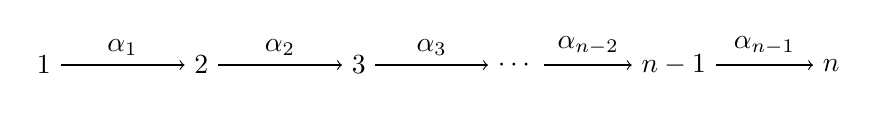
\begin{tikzpicture}
         \node (A) at (0,0) {1};
         \node (B) at (2,0) {2};
         \node (C) at (4,0) {3};
         \node (D) at (6,0) {$\cdots$};
         \node (E) at (8,0) {$n-1$};
         \node (F) at (10,0) {$n$};
         \draw[->] (A) -- (B) node[midway, anchor=south] {$\alpha_1$};
         \draw[->] (B) -- (C) node[midway, anchor=south] {$\alpha_2$};
         \draw[->] (C) -- (D) node[midway, anchor=south] {$\alpha_3$};
         \draw[->] (D) -- (E) node[midway, anchor=south] {$\alpha_{n-2}$};
         \draw[->] (E) -- (F) node[midway, anchor=south] {$\alpha_{n-1}$};
      \end{tikzpicture}
   \end{center}
   Tested using \texttt{IsFractionalCalabiYau}
   \begin{multicols*}{2}
      \begin{center}
         \begin{tabular}{|c|c|c|}
            \hline
            $n$ & Ideal & Syzygy \\
            \hline 
            3 & $(a_1a_2)$ & 6 \\
            \hline
            4 & $(a_1a_2)$ & 8 \\
            & $(a_2a_3)$ & 8 \\
            & $(a_1a_2, a_2a_3)$ & 8 \\
            & $(a_1a_2a_3)$ & 10 \\
            \hline
            5 & $(a_1a_2)$ & 10 \\
            & $(a_2a_3)$ & 10 \\
            & $(a_3a_4)$ & 10 \\
            & $(a_1a_2, a_2a_3)$ & 10 \\
            & $(a_1a_2, a_3a_4)$ & 10 \\
            & $(a_1a_2, a_2a_3, a_3a_4)$ & 10 \\
            & $(a_1a_2a_3)$ & 14 \\
            & $(a_2a_3a_4)$ & 14 \\
            & $(a_1a_2a_3, a_2a_3a_4)$ & 14 \\
            & $(a_1a_2a_3a_4)$ & 14 \\
            \hline
            6 & $(a_1a_2)$ & 12 \\
            & $(a_2a_3)$ & 12 \\
            & $(a_3a_4)$ & 12 \\
            & $(a_4a_5)$ & 12 \\
            & $(a_1a_2, a_2a_3)$ & 12 \\
            & $(a_1a_2, a_3a_4)$ & 12 \\
            & $(a_1a_2, a_4a_5)$ & 12 \\
            & $(a_2a_3, a_3a_4)$ & 12 \\
            & $(a_2a_3, a_4a_5)$ & 12 \\
            & $(a_3a_4, a_4a_5)$ & 12 \\
            & $(a_1a_2, a_2a_3, a_3a_4)$ & 12 \\
            & $(a_1a_2, a_2a_3, a_4a_5)$ & 12 \\
            & $(a_1a_2, a_3a_4, a_4a_5)$ & 12 \\
            & $(a_2a_3, a_3a_4, a_4a_5)$ & 12 \\
            & $(a_1a_2, a_2a_3, a_3a_4, a_4a_5)$ & 12 \\
            \rowcolor{red!30!white}
            & $(a_1a_2a_3)$ & 9 \\
            \rowcolor{red!30!white}
            & $(a_2a_3a_4)$ & 11 \\
            \rowcolor{red!30!white}
            & $(a_3a_4a_5)$ & 9 \\
            \rowcolor{red!30!white}
            & $(a_1a_2a_3, a_2a_3a_4)$ & 9 \\
            \rowcolor{red!30!white}
            & $(a_1a_2a_3, a_3a_4a_5)$ & $>30$ \\
            \rowcolor{red!30!white}
            & $(a_2a_3a_4, a_3a_4a_5)$ & 9 \\
            \rowcolor{red!30!white}
            & $(a_1a_2a_3, a_2a_3a_4, a_3a_4a_5)$ & 22 \\
            \rowcolor{red!30!white}
            & $(a_1a_2a_3a_4)$ & 22 \\
            \rowcolor{red!30!white}
            & $(a_2a_3a_4a_5)$ & 22 \\
            \rowcolor{red!30!white}
            & $(a_1a_2a_3a_4, a_2a_3a_4a_5)$ & 22 \\
            \rowcolor{red!30!white}
            & $(a_1a_2a_3a_4a_5)$ & 9 \\
            \hline
            \rowcolor{red!30!white}
            8 & $\ell_2$ & 16 \\
            \rowcolor{red!30!white}
              & $(a_1a_2, a_2a_3, a_3a_4, a_4a_5, a_5a_6, a_6a_7)$ & 8 \\

         \end{tabular}
      \end{center}
   \end{multicols*}
\end{flushleft}
\end{document}
